\chapter{Accelerator Generation and Integration Using Program Binaries}
\label{instrumentChap}
As usability remains to be one of the most significant obstacles for adopting FPGA computing, in this chapter, we explore the possibility of a user
transparent flow for mapping applications to systems with reconfigurable components.
Contrast with previous chapters where source codes in high level
languages are used as inputs, here we try to only use the program binaries and their runtime profiles as the design entries. 
The mechanism for integrating the accelerator back into the overall program execution is also examined. While the synthesis and tuning of the computational pipeline was an attempt to create better accelerators running on FPGA itself, in this chapter, we
further discuss the interaction between the software component and the FPGA accelerators. From the users' perspective, a flow based on
program binaries requires no source rewriting
nor recompilation, the effort needed to take advantage
of the reconfigurable platform is thus minimized. 

\section{Characteristics of the Targeted Platform}
\label{chartarg}
The general approach of translating program binaries to accelerators can certainly be applied to various heterogeneous platforms. To justify some of the design decisions made in our flow, the assumed platform 
characteristics need to be outlined first. 
In section~\ref{hetero}, a whole array of machines with reconfigurable
components were examined and there is a wide spectrum of configurations
when it comes to how tightly integrated the reconfigurable fabric is to
the processor. 
In this work, we focus on the part of the space where the general purpose processor and the reconfigurable component are loosely coupled.
Instead of being a functional unit in the processor
execution pipeline, the FPGA is used as a coprocessor for which
communication and management is assumed to be expensive.
Meanwhile, the capacity of the reconfigurable fabric can potentially be greater as it is not constrained in any way by the pipeline of the associated processor. 
Most of the off-the-self systems currently available or in development~\cite{xeonwithfpga} fall into this category. As the
costs of semiconductor manufacturing become prohibitive, 
special processors with modified pipeline accommodating
reconfigurable functional units are less likely to be built
and offered commercially, as compared to systems with conventional
processor and FPGA integrated at either chip, package or board level.

Another important factor to consider is how sharable the memory
is between the CPU and the FPGA. 
One possible configuration, as represented by the zynq SoC, has
the CPU's address space shared with the programmable logic.
The physical addresses used to access the memory are identical,
whether it comes from the CPU or the FPGA. Of course in the presence
of virtual memory, address translation needs to occur within the FPGA
before memory requests are sent out. On the other hand, there are
platforms where the FPGA has its own memory space which is
explicitly populated with the working dataset before the activation of 
the accelerator~\cite{sdaccel}. It's worth noting that this difference in programming model
is orthogonal to the actual physical configuration of the platform. For instance, CPU and FPGA located in two different sockets can have shared address space while a system based on a single chip SoC may associate the FPGA with a separate DRAM interface which are not directly
accessible by CPU. 
Given the flexibility of FPGAs, there are certainly ways to create a layer of abstraction conforming to either one of these schemes, regardless
the original expected usage model. However in this work, we 
do not make assumption about the underlying platform and try to
 devise a mechanism for each scheme. 
%we treat these
%two schemes differently, as will be discussed in section~\ref{makingAcc}.
Finally, in any CPU+FPGA coprocessor systems, the access of data memory by the programmable logic can be seen as adding to the communication overhead between the
accelerated part and the software components, which is a key parameter
in determining if a part of the program should be accelerated using hardware.



\section{Acceleratable Regions In Program Binaries}
The trade-off between communication efficiency and capacity
in the reconfigurable components of the systems dictates
the granularity of the accelerators to be synthesized. 
Given the loose coupling between the programmable logic and the processor,
while it is still possible to create accelerators for small windows of dynamic instruction stream, the cost of frequently controlling and communicating
with these tiny hardware engines would nullify any performance gain
achieved. 
It is ideal to have a relatively large chunk of computation
handed off to the FPGA, which then works independently with little
intervention from the CPU, before signalling the completion of the task.
The natural targets for our flow are therefore loop nests in the program
binaries. To find the loops, we use the DyninstAPI~\cite{dyninst} to parse through
the program binaries and construct the control flow graph (CFG). There may be cases where code segments are shared by multiple loops, making it harder to statically carve out the best code region for acceleration. For these
scenarios, we leverage can runtime profile of the program to find the prevalent
loops and extract single-entry-multiple-exit loops which can undergo further
optimizing transformations. 
Meanwhile, due to the presence of statically unresolvable control flow, e.g. indirect jump,
not every part of the program can be analyzed. Several techniques were
proposed to tackle this in dynamic binary translation~\cite{}, which we can potentially
adopt. However, we do not aim to have complete coverage of the code as only the
computation heavy loops are of interest to us.
Practically speaking, the more regular loops, which are the ideal candidates for FPGA acceleration, are generally easy to detect and analyze. 
% The accelerator will be invoked only if the execution 


Another characteristic of the FPGA platform is its low clock frequency
(as compared to a typical CPU), thus to have significant speed up, there
needs to be substantial amount of parallelism extracted, which requires large windows of instruction.
In addition to instruction level parallelism within basic block or a single iteration of a loop, coarse grained parallelism 
%spanning the iteration space of loop nests 
also needs to be exploited. Blocks of loop iterations are to be executed in parallel, which implies very aggressive instruction
reordering when the accelerators are created.
%
%Meanwhile, the aggressive reordering of these instructions in creating the %accelerator
%makes any speculative execution very expensive. 
Consequently, speculative execution, which some binary-based dynamic parallelization techniques were based on, may become rather expensive. As states generated by the speculatively performed operations need to be buffered, 
the amount of space required to accommodate the massively parallelel execution engine
%exploited
can be large.
The subsequent commit of these state may also induce long delay
or require complicated hardware mechanism.
In particular, for any speculatively disambiguated memory accesses, the address streams need to be dynamically cross compared to ensure the
reordering of loads and stores are indeed valid. 
Using runtime profile can boost the confidence with which the disambiguation
is performed, but the probabilistic nature of the approach does not
relieve us the need for costly dynamic checking mechanisms. To generate
lean and fast accelerators, in this work, we try to extract a set of conditions for parallelization which does not vary with the amount of work
in the loop. In other words, we want to find computation that can 
be done in run time with a fixed, statically known cost, yet still guarantees the validity of the instruction reordering we have performed for accelerator generation. 
%This will allow us to quickly gauge if an instance of a loop nest should be executed on hardware.

\subsection{Dependencies in Loops}
To understand what characteristics a loop nest should manifests for it to be a feasible target, it is useful to start from the theory of loop dependence. As
explained in section~\ref{sec:partins}, statements cannot be parallelized or
reordered when there are RAW, WAR or WAW dependencies between them. In the context of instructions in loop nests,~\cite{Kennedy:2001:OCM:502981} defined
loop-carried and loop-independent dependencies between a pair of statements $S_1$ and $S_2$ (at least one of which is writing to memory):
\begin{itemize}
    \item Loop-carried dependency: $S_1$ accesses a common memory location 
    on one iteration of a loop, and $S_2$ accesses the same location on a subsequent iteration. 
    \item loop-independent dependency: $S_1$ and $S_2$ access the same memory location in the same loop iteration, and there is a execution path from $S_1$ to $S_2$. 
\end{itemize}
The concepts of \textit{iteration number}, \textit{iteration vector} and \textit{iteration space} were also introduced. The iteration number is the 
index number for a particular loop iteration, while the iteration vector
extends this concept to a multi level loop nest. Each element in the vector
corresponds to one level in the loop nest with left most element representing the outermost loop index. The set of all possible iteration vectors then
constitute the iteration space. Figure~\ref{fig:inivis} visualizes these concepts with a simple loop nest. 

\begin{figure}[htp]
\begin{center}
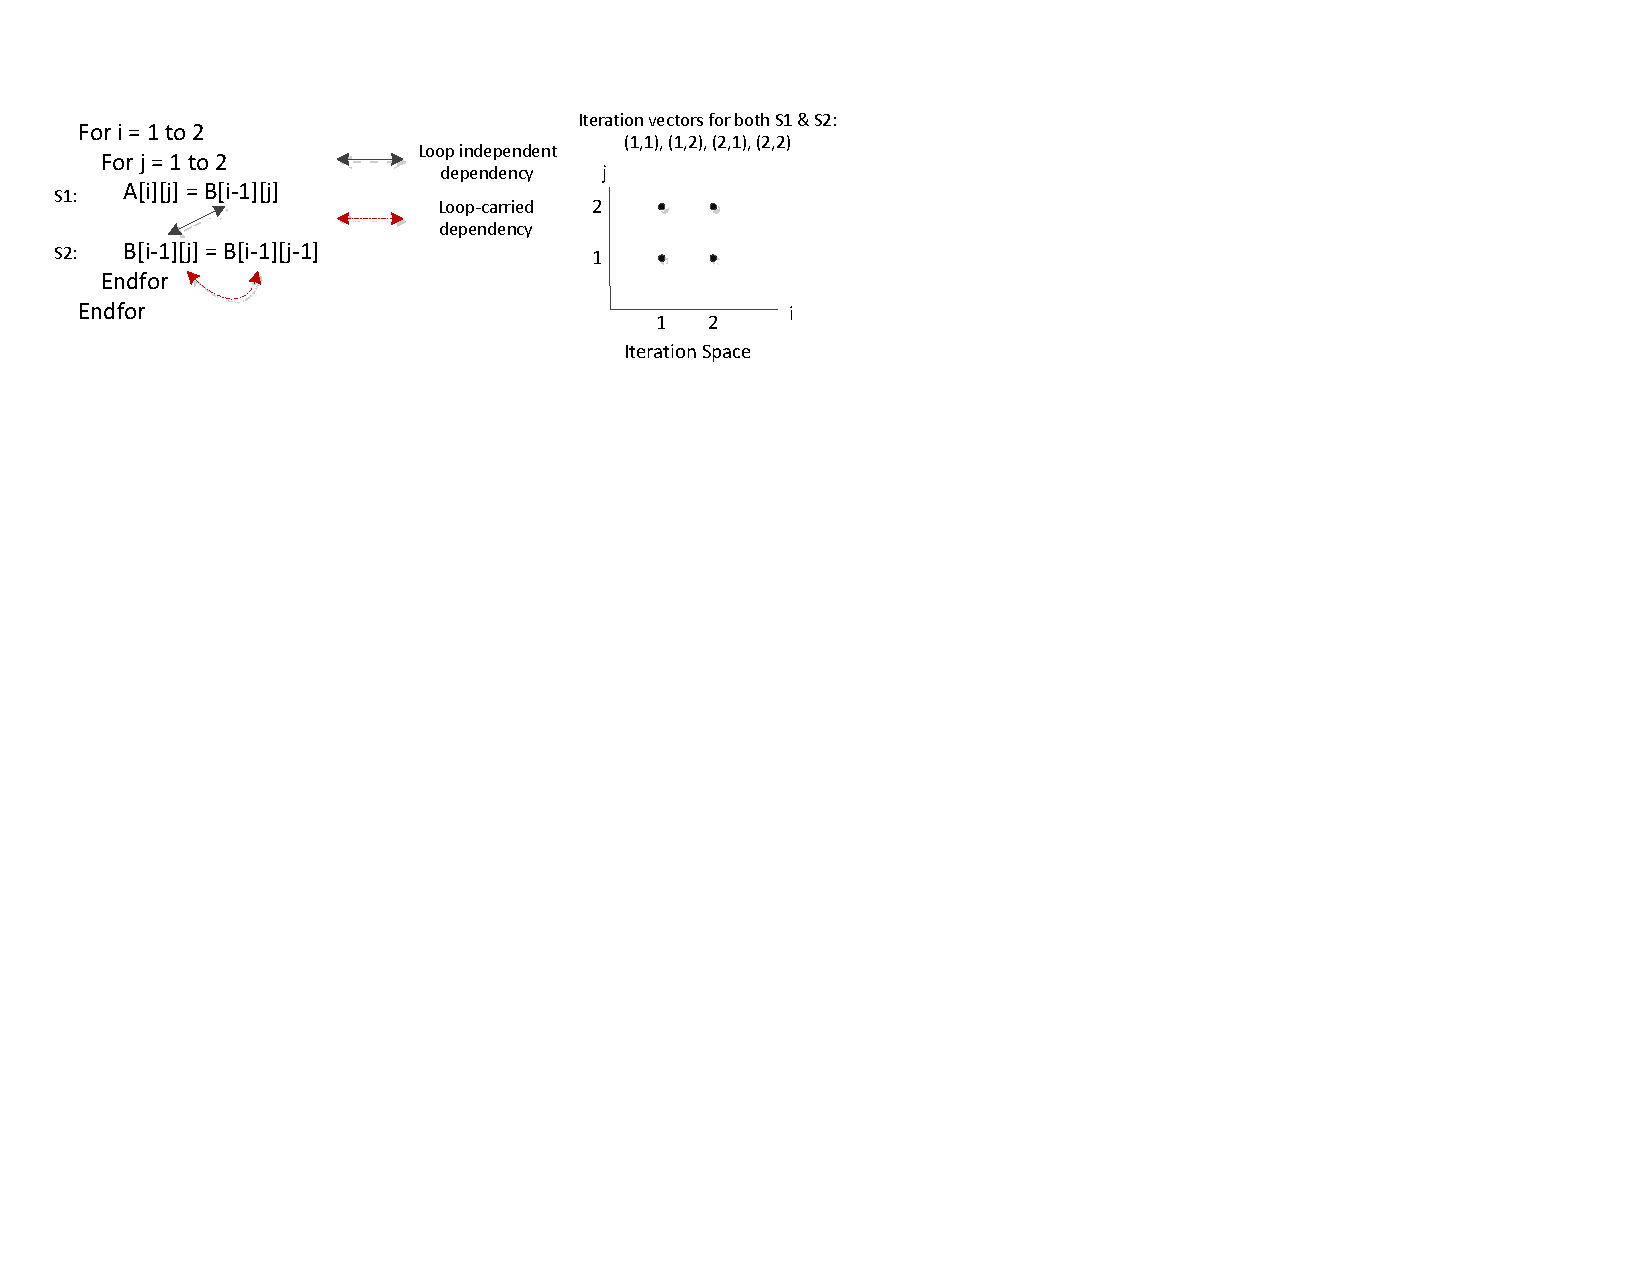
\includegraphics[width=0.9\linewidth]{chap6fig/iterationSp.pdf}
\caption{Dependencies in a Loop Nest
\label{fig:inivis}}
\end{center}
\end{figure}

To exploit coarse grained parallelism in the loop nest, we need to ensure the
absence of loop carried dependencies at a particular level in the loop nest. There are also simple transformations(e.g. loop interchange) which can move loop carried
dependencies to other loop levels so only loop-independent dependencies are left. To enable the discovery of these opportunities, we need to find, in each statement's iteration space, if they intersect with other statements' accessed memory locations. In general, the memory addresses to be accessed can be arbitrary functions of loop indices and runtime data, which makes it impossible to statically determine if
dependencies exist. There are, however, a large set of problems where
the memory referenced can be analyzed during compile time as the addresses are affine functions of the loop index variables. For loop nests of this kind,
dependency analysis is essentially finding integer solutions for the problem:

\begin{equation}
\begin{aligned}
\label{dioeq}
& \text{} & & f(\vec{x}) = h(\vec{y}) \\
\end{aligned}
\end{equation}
\begin{equation*}
\begin{aligned}
& \text{ where}  & & f(\vec{x}) = a_0 + a_1x_1+...+a_nx_n \\
& & & h(\vec{y}) = b_0 + b_1y_1+...+b_ny_n \\
& & & \vec{x}_{lb} \le \vec{x} \le \vec{x}_{ub} \\
& & & \vec{y}_{lb} \le \vec{y} \le \vec{y}_{ub}
\end{aligned}
\end{equation*}
Or equivalently this linear Diophantine equation:
\begin{equation}
\begin{aligned}
\label{adioeq}
a_1x_1-b_1y_1+...+a_nx_n-b_ny_n = b_0 - a_0
\end{aligned}
\end{equation}
\begin{equation*}
\begin{aligned}
& \text{ where}  & & x_{lb}_k \le x_k \le x_{ub}_k \\
& & & y_{lb}_k \le y_k \le y_{ub}_k \\
\end{aligned}
\end{equation*}

Both function $f$ and $h$ takes a iteration vector from within the iteration space of the statement, bounded by $\vec{x}_{lb}/\vec{y}_{lb}$ and $\vec{x}_{ub}/\vec{y}_{ub}$, and map it to a memory location. When
multi-dimensional arrays are used, variables can be separated such that
we have multiple simultaneous equations which are simpler to solve.
The loop carried dependency in figure~\ref{fig:inivis}, for instance, correspond to the following equations:
\begin{equation*}
\begin{aligned}
-1+x_1 = -1+y_1 \\
x_2 = y_2-1 \\ 
\end{aligned}
\end{equation*}
\begin{equation*}
\begin{aligned}
& \text{ where}  & & 1 \le x_1 \le 2 \\
& & & 1 \le x_2 \le 2 \\
& & & 1 \le y_1 \le 2 \\
& & & 1 \le y_2 \le 2 \\
& & & x_1,x_2,y_1,y_2 \in Z
\end{aligned}
\end{equation*}


This problem is an integer linear program, one of the NP-complete problems.  
There are various techniques~\cite{banerjee}~\cite{gcd}, proposed over the years, to efficiently solve a relaxed version of this problem. 
%can be used to compute if
%dependencies exist between memory references. Essentially they are all trying %to find solutions for the problem:
%Many techniques were proposed for compiling these problems onto variable %processors. 
In our binary-based flow, we also try to target these analyzable loop nests, some of which are especially amenable to FPGA acceleration. 
Identifying these regions from the program binaries, however, is not as
simple as doing it from the source code.


%This can be done by solving the

%direction vector
%is the way to do it
%To capture the dependencies between statements, \texit{direction vector} are computed between statements.

\subsection{Challenges for Binary-based Analysis}
\label{sec:cfbba}
The regular and analyzable memory access patterns expressed in high
level languages become rather mangled when the program binaries are 
being examined. All memory accesses are pointer based with no high
level information to indicate if the data structures they are targeting
are disjoint. With dimensionality of the arrays eliminated, 
separate variables in original address calculation are now coupled to each other. In essence, we have to perform dependency analysis on a huge linear
array with all all addresses being the result of some run time computation.
Figure~\ref{fig:mangledMem} illustrates how different a
set of memory accesses manifest themselves in the actual high level source code v.s. program binaries.

\begin{figure}[htp]
\begin{center}
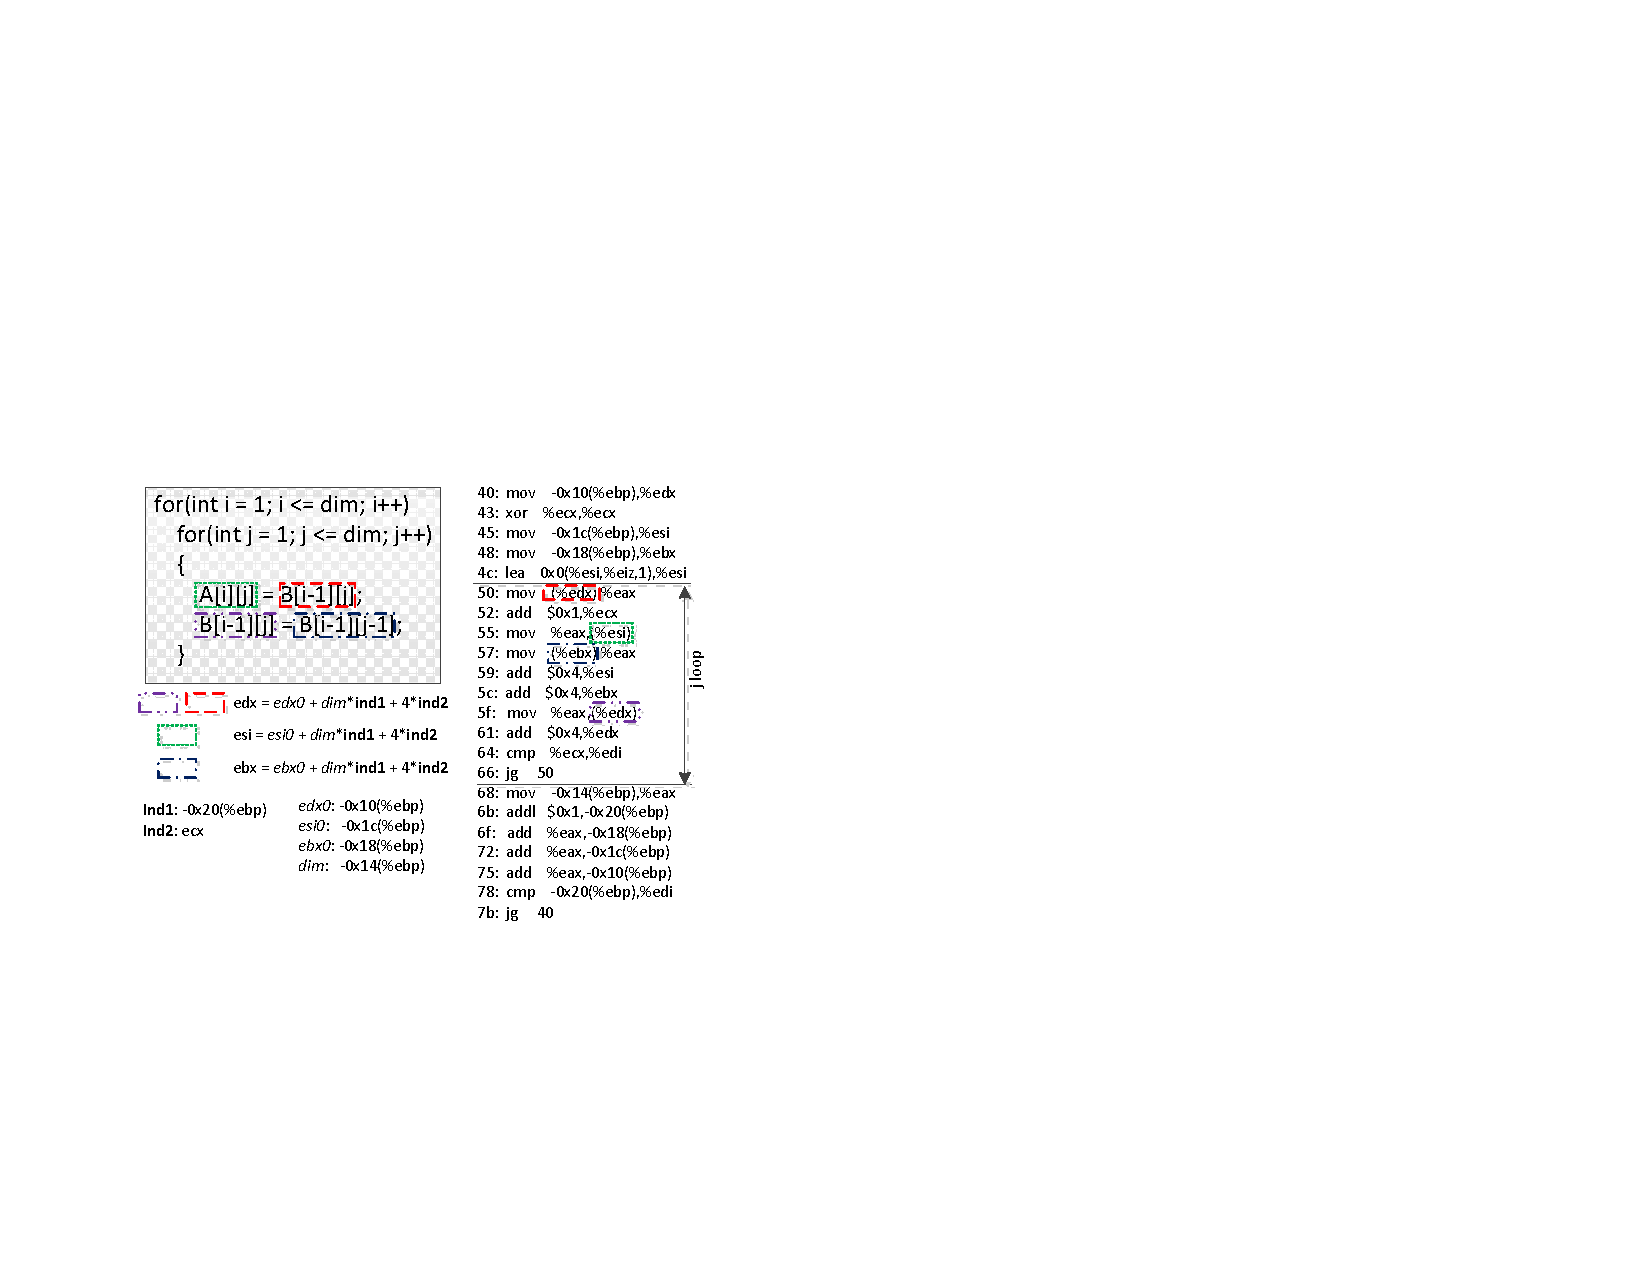
\includegraphics[width=0.8\linewidth]{chap6fig/memBin.pdf}
\caption{Memory Accesses in Program Binaries
\label{fig:mangledMem}}
\end{center}
\end{figure}

In this example, even though the original array references are all affine functions of the loop index variables, in the program binaries, their calculation is much more complex. 
Dependency testing involving only a single loop index in the source code now have to deal with multiple induction variables. More importantly, for equation~\ref{adioeq}, the coefficients ($a_0...a_n$ and $b_0 ... b_n$) are statically known constants while
in the binaries, everything is a runtime data item stored in either a register or a memory location. Naively 
substituting these symbolic variables into the Diophantine's equations yields
a non-linear formulation which can not be solved by the common techniques
in optimizing compilers. On the other hand, %it is relatively straight forward, 
as long as these coefficients are unchanged during the execution of the loop nests, we can leverage various classic dependency testing techniques to formulate a fixed set of checks to be performed during run time. This is possible because the dependency
analysis problem does not scale up with the number of iterations, but rather the number of levels in the loop nest, which is easily recognizable from the static binaries. We therefore can quickly verify our coarse grained parallelization before the invocation of the accelerator, 
avoiding speculative execution and the associated costs. 

In our flow, dataflow analysis is always performed on loop nests to ensure there are no updates to these coefficients during the loops' execution, before more detailed dependency testing and parallelization are attempted. The  potential for actual speed up of course largely depends on the existence of coarse grained parallelism.



%we can be sure that only a fixed amount of computation is needed in
%the dependency. This is not hard to see as the size of the problem formulated 
%does not depend on the actual values of the variable but the number of levels in the loop nest.

%we can assume they are runtime constant and the dependency analysis
%can be carried out. 



%Our approach to deal with this uncertainty is described later in section~\ref{makingAcc}.





\subsection{From Dependency Testing to Parallelization}
\label{sec:fdtp}
%With the dependency testing done, we need to examine the loop nests' potential for parallelization.

To identify the opportunities in parallelizing a loop nest, the dependency distance and direction vectors~\cite{opac-b1000180} are used.
%One way to bridge this gap is through the use of distance and direction vectors~\cite{opac-b1000180}. 

\begin{figure}[htp]
\begin{center}
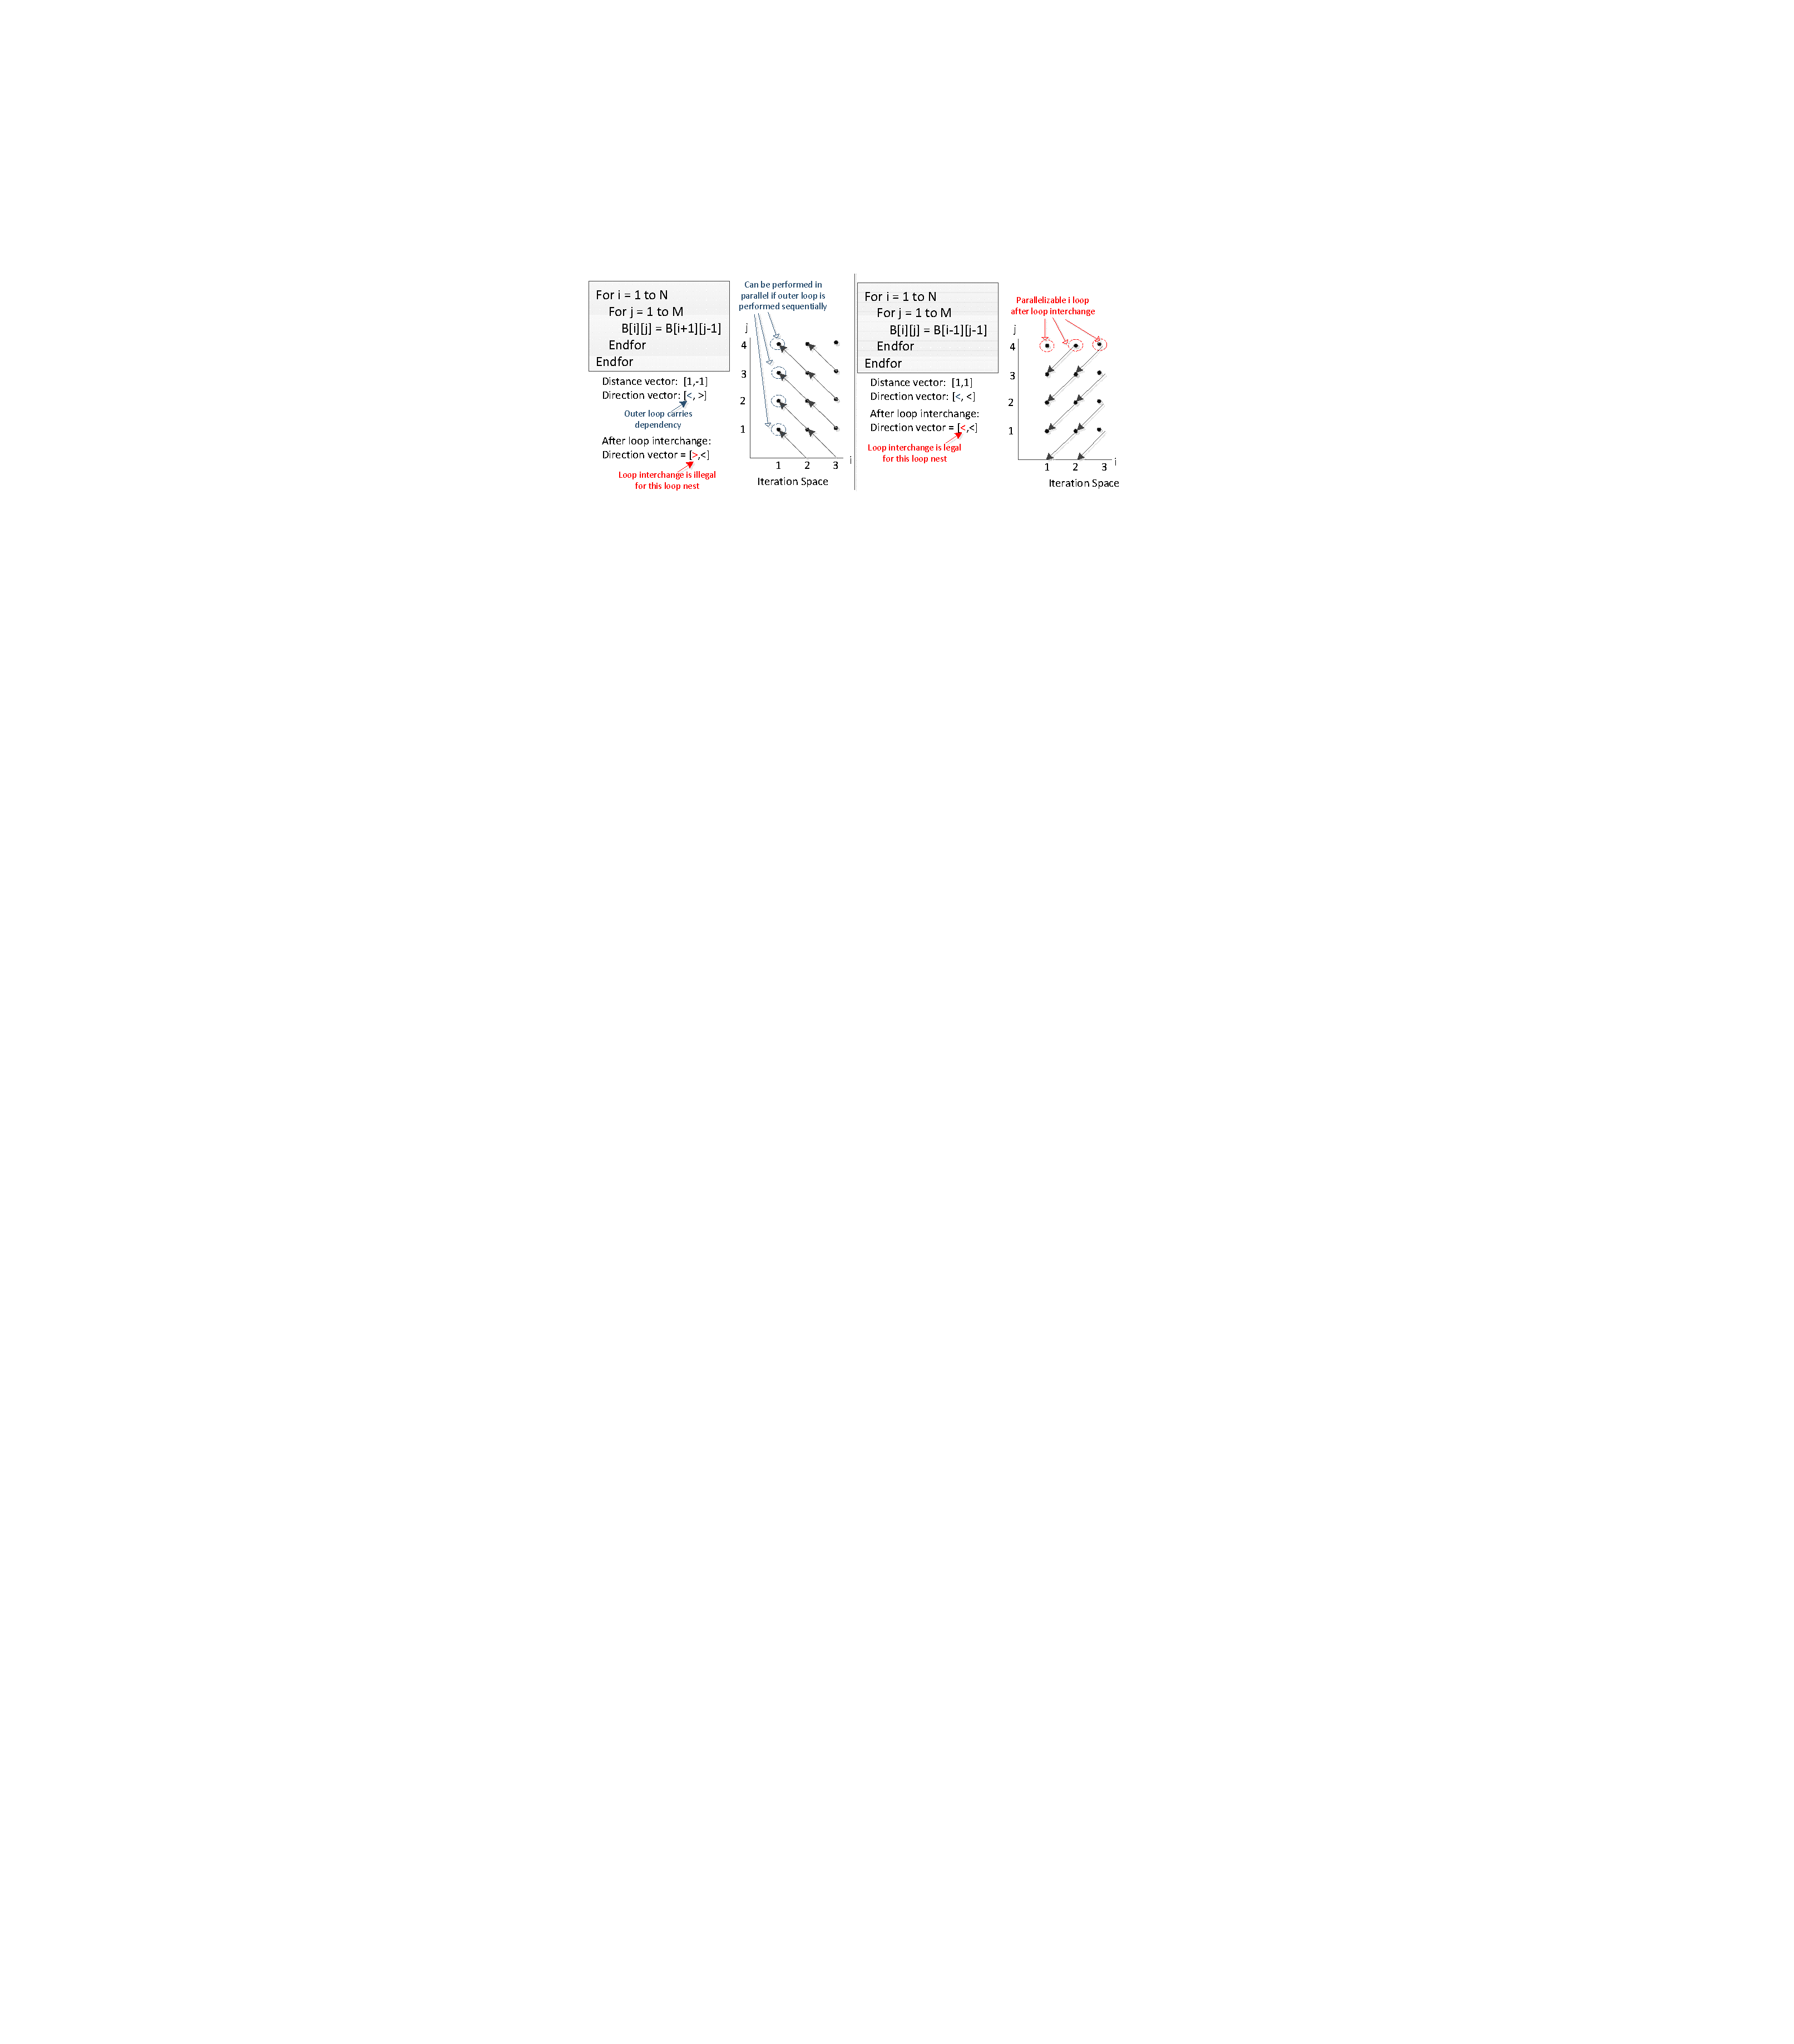
\includegraphics[width=1.0\linewidth]{chap6fig/paral.pdf}
\caption{Parallelization with Direction Vectors
\label{fig:paral}}
\end{center}
\end{figure}
The dependence distance vector can be computed:
\begin{equation*}
\begin{aligned}
&  & & \vec{d}(\vec{x},\vec{y}) = \vec{y}-\vec{x} \\
& \text{ where }&   & \vec{x} \text{ and }\vec{y} \text{ are solution to equation~\ref{dioeq}}  
\end{aligned}
\end{equation*}

The distance vectors give rise to direction vectors $D(\vec{x},\vec{y})$:
\begin{equation*}
\begin{aligned}
  & & ``<" \text{ if } \vec{d}(\vec{x},\vec{y})_k>0 \\
 \vec{D}(\vec{x},\vec{y})_k = &   & ``=" \text{ if } \vec{d}(\vec{x},\vec{y})_k=0\\
 & & ``>" \text{ if } \vec{d}(\vec{x},\vec{y})_k<0
\end{aligned}
\end{equation*}


The convention is to have the lexicographically earlier iteration vector to be
$\vec{x}$ and with that the leftmost non-``=" element of a direction vector would always be ``$<$". 
The index for this leading ``$<$" is also the level of the  loop-carried dependency. 
Assuming a transformation $T$ does not violate loop-independent dependencies,
~\cite{Kennedy:2001:OCM:502981} proved that $T$ is valid as long as
it does not cause some of the direction vectors to have ``$>$" as the leftmost non-``=" component. In addition, any iteration reordering at a level of the loop not carrying dependency is also valid. Using these proven theorems, we can
decide if loop transformations and iteration parallelization are legal when we know all the direction vectors of a loop nest. Figure~\ref{fig:paral} illustrates a
few scenarios where dependency direction vectors are used to determine validity
of transformation/parallelization.








%To summarize, our flow targets loop nests whose direction vectors can be extracted and coarse grained parallelism identified.



\begin{comment}

we leverage several techniques for taking advantage of the discovered parallelism. For the inner most loop, loop pipelining is always applied
to 

Assuming a particular loop level does not carry dependency, 

Comparing against other parallel computers such as multicore or SIMD machines, the 

Parallelization in FPGA vs others:
vectorization ? separate thread? loop pipelining? 


In order to get the dependency vector however, the memory access patterns would
need to be analyzable. Techniques for extracting dependency vectors were outlined in the .... These techniques generally require the array references
to be affine functions of the loop indices, where the coefficients are
all constants. 
Unfortunately, in the case of accelerating binaries, the coefficients are 
always variables stored in either register or a memory location. Naively
substitutes these variable into the Diophantine's equations yield
non linear conditions...As a result, even if the underlying computation are parallelizable, it is a lot harder to verify with the program binaries
as the starting points. It is relatively straight forward, however,
to detect if these coefficient are changed during the execution of the loop nests. 
\end{comment}

% we want something analyzable ---- % but of course even if the source code
% is analyzable, the binary may not be


\begin{comment}
Schemes for checking 
%

This is certainly compatible with the how conventional FPGAs are used
in most applications, where entire compute intensive loops are offloaded
and sped up.

Even as we focus on speeding up loops with large iteration count,
certain loop nests are just difficult to accelerate using FPGAs.
%especially
%when all higher level information is stripped away, as is the case with program binaries.
Due to the slower frequency of FPGA accelerators, it is not sufficient to just exploit instruction level parallelism. For there to be any net gain
in performance, coarse grained parallelism at the loop level has
to be extracted. To establish independence between different loop iterations or perform transformation to extract coarse grain parallelism, the 
\end{comment}



\section{A Two Phased Approach for Accelerating Program Binaries Using FPGA}
\label{makingAcc}
As the accelerator synthesis, which also includes the traditional FPGA CAD flow,
can take hours to finish, the loop transformation/parallelization need to be performed offline. We therefore have to obtain the direction vectors 
before running the actual program. 
In this work, Banerjee's test~\cite{banerjee} is used to find these vectors. The required coefficients for equation~\ref{adioeq} are extracted from past runtime profiles. The dependency testing and parallelization performed during this \textit{offline phase} are  thus a reflection of the programs' past behavior. When the accelerator is actually running, the input data would have changed. The \textit{online phase} thus includes a mechanism to guarantee the 
semantics of the program is not violated by the reordering performed during
the accelerator synthesis. As we have mentioned in section~\ref{sec:cfbba},
a verifying function is invoked before the accelerator, ensuring the correctness
of the overall execution. 


This online phase test is also one of the reasons why we choose Banerjee's method for our dependency testing.
Banerjee's inequality tests for existence of any real solutions for the Diophantine's equations. Since it only tackles the non-integer relaxation of the ILP formulation, the results obtained are conservative.
It will never report lack of dependencies when one exists,  but may report false dependencies, i.e. when all the real solutions are non-integral.
 More accurate tests like~\cite{omega} find integer solutions but are more costly. Since we are
going to perform the test again using runtime data when the accelerator is actually
being invoked, the faster, though more pessimistic, method is preferred.



\subsection{Offline Phase: Parallelization and Accelerator Synthesis}



When FPGA accelerators are synthesized through HLS, several techniques are used to exploit
the coarse grained parallelism. For the inner most
loop, it is generally very cost effective to pipeline the loop. If
the iterations are parallelizable, the initiation interval would be 1.
Assuming there are $M$ iterations, the total execution time of the loop
would roughly be $M$ cycles. To further reduce this number, loop unrolling
can be performed. It combines multiple iterations into one, effectively
turning inter-iteration parallelism into fine grained parallelism. 
The iteration count is reduced by the unroll factor ($U$) while the II does not change. Consequently, the total execution time is reduced to roughly $M/U$ cycles with a approximately $U$ fold increase in area. 

\begin{figure}[htp]
\begin{center}
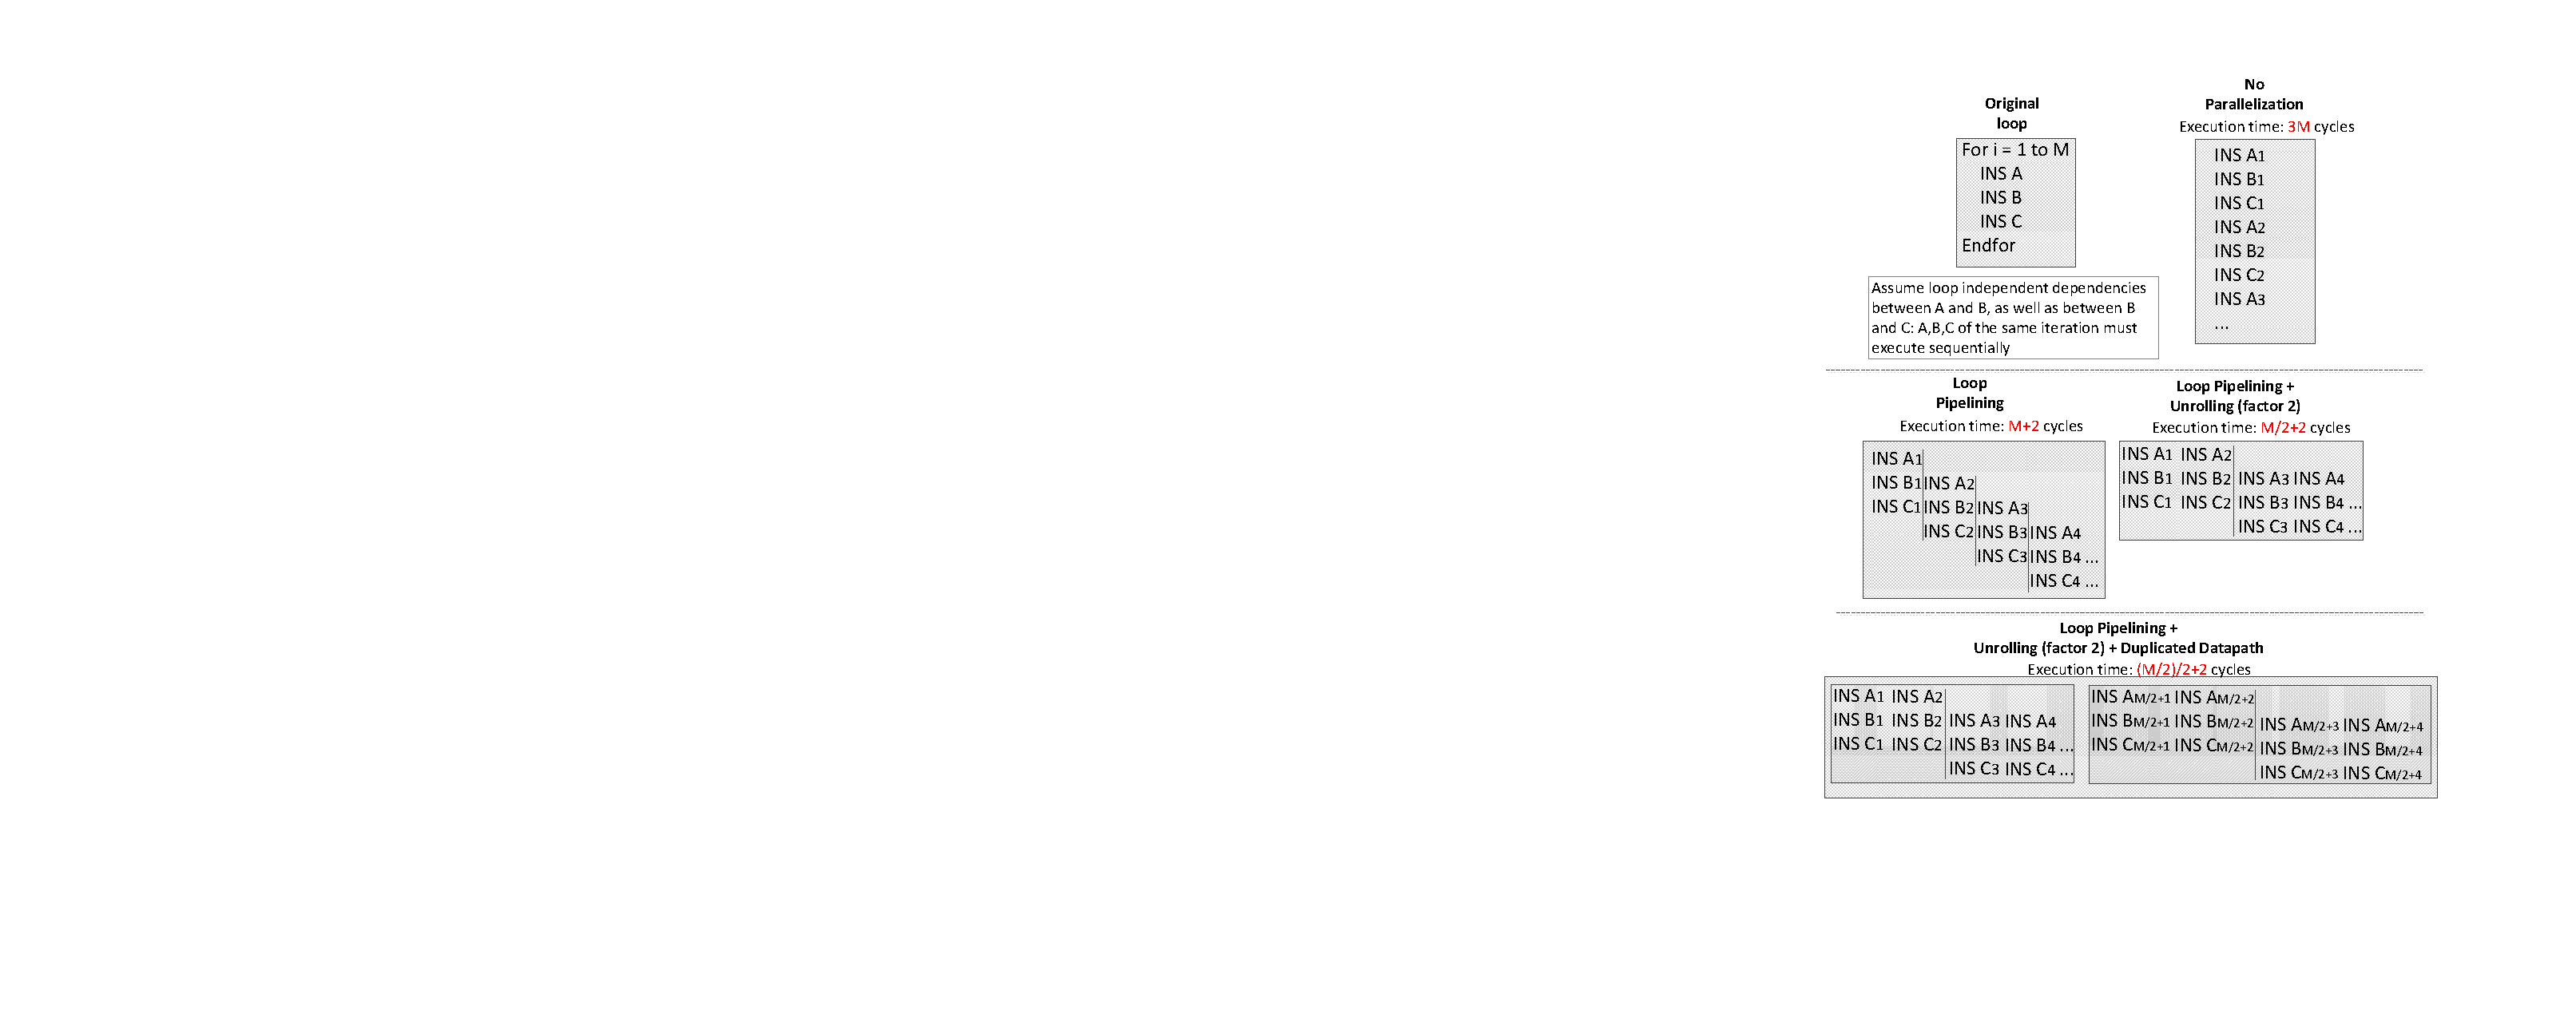
\includegraphics[width=0.7\linewidth]{chap6fig/fpgaParallel.pdf}
\caption{Parallelization in FPGA Accelerators
\label{fig:fpgaparal}}
\end{center}
\end{figure}

To improve the throughput of the accelerator even further, multiple
independent datapaths can be instantiated, each performing a subset of 
the iterations. This technique can be used to parallelize outer loops
as well. For loop with a large number of iterations, this technique provides a good way to trade off more on-chip resources for better performance, although
it also incurs some extra synchronization overheads. Another advantage of
having multiple datapaths is the independence between their controllers.
In an earlier chapter(section~\ref{motex}), we illustrated the vulnerability
of a single monolithic schedule to data access latencies and the resulted
underutilization of the memory bandwidth. In the presence of coarse grained parallelism, it is much easier to fully exploit the data bandwidth provided
by the platform, as each datapath independently generates requests, whether
its peers are stalled or not. 
Certain platforms also provide multiple channels
for off-chip memory access, which can be more easily utilized with duplicated datapaths.
Figure~\ref{fig:fpgaparal} illustrates the described parallelization schemes for FPGA accelerators.

We can draw similarities between these techniques and the compiler optimizations targeting architectural features
of various parallel processors. Loop pipelining was a scheduling technique
widely used for VLIW machines, where it is often called software pipelining. Loop unrolling, in the synthesis of FPGA
accelerators, is similar to vectorization, as a wider processing engine
is now used to process multiple iterations simultaneously. The replication of
datapath is essentially generating multithreaded implementation from a serial
specification. Previous research in automatic parallelization can thus be
leveraged for our flow. In this work, we are not trying to invent new techniques, but to enable past work to be applied to program binaries on FPGA
platform. 

While FPGAs can exploit parallelism in 
multiple different ways, another important aspect to optimize for would be the temporal and spatial locality of data access. While multiple datapaths can
easily saturate the offchip memory bandwidth, there might be wastage if opportunities for data reuse are missed. 
Even in the absence of data reuse, requests for 
contiguous segments or memory locations close to each other are more efficiently served by the caches and the memory subsystem.
In our parallelization engine, we try to increase the ratio of computation per unit of data communicated with off-chip RAM. By performing loop interchange under the dependency constraints, we can generate multiple versions of a loop nest. To find the implementation with best locality, we would like to have the version with the smaller
memory footprint (normalized by iteration count) at the inner loop level.
For our targeted loop nests, the memory addresses accessed are affine expressions of the loop index variables. The coefficient for each of them
decides how large of a stride each iteration takes, which conveniently
approximate how ``unlocal" the memory accesses are. 
Thus for a particular loop index variable, the smaller the coefficient, the deeper its corresponding loop level should go.
This is illustrated in figure~\ref{localityopt}. 

The algorithm used in our parallelization engine is outlined in algorithm~\ref{algoPara}. This is a modified version of the \textit{codegen}
procedure from~\cite{Kennedy:2001:OCM:502981}, which targets vector machines.
Our implementation, in addition to data level parallelism, also try to expose
thread level parallelism at the outer level loop, which can then be easily exploited by multiple FPGA datapaths. 
The results from our algorithm only provides a starting point for the design space exploration. Even for a single vectorized instruction, combinations of techniques illustrated in figure~\ref{fig:fpgaparal} can be applied to
produce implementations of different performance area trade-off. Meanwhile, 
the supporting infrastructure on the FPGA can also be modified on a per
application basis. The parametrization of on-chip buffer, communication mechanism with external
storage etc. are all parts of the design space. The co-tuning of these ``glue"
structures in conjunction
with the accelerator itself is left to future work.  In section~\ref{biev}, we sample a small subset of the possible design points
to show the trade-off between different metrics.


There are also other transformations which can be applied to extract additional parallelism or to achieve better data reuse. Loop fission and loop tiling, for instance, are techniques used in some optimizing compilers. 
Their incorporation is certainly feasible with our general approach and will
add more dimensions to the design space. 

The actual implementation of the parallelization engine is built
on top of the LLVM framework. As LLVM takes C/C++ as input, we created a preprocessing step
to convert the program binary to C functions. It is also in this step when we extract
coefficients for the Diophantine equation and bounds for loop indices from past runtime profiles.
The numbers obtained are substituted as constants into the C functions, enabling the subsequent analysis. 
In the original binaries, these variables are often stored in the memory. 
Thus in addition to examining their past values, we also perform a check to ensure their memory
locations do not alias with any other references performed by the loop nest, again using the
addresses observed from the profile. Most of the time, these locations can be
recognized as part of the call stack, and are normally completely disjoint from
the memory footprint of the actual loop. We can thus easily disambiguate them using a simple
range test. Of course, when the accelerator is actually being invoked, this test would need to be
run again, as will be detailed in section~\ref{onlinephase}.
FIXME:There are many existing compiler passes within LLVM which facilitates the analysis ....
After the transformations, the LLVM IR is converted back to C, before HLS is used
to generate the final circuits. Multiple independent C functions can be generated
when multiple datapaths are desired in the final implementation. Vendor specific
pragmas are also inserted to provide guidance for the HLS tool. An example output,
which targets Vivado HLS backend, is shown in figure~\ref{}. 



\begin{comment}
c 2 c
independnet


Even though their location can usually be recognized 
as part of the call stack, we still check for aliasing between 


There are various transformation (e.g. loop interchange passes already
built into LLVM
\end{comment}
%In this work, however, we aim to 

%In addition, as the hardware on FPGAs can be parameterized on a per application basis, there is a huge design space where the high level input
%for HLS as well as the supporting infrastructure (e.g. on chip buffer) can
%be co-tuned. A thorough exploration of this space is left to future work.

%are affine expression of the loop indices, each with a different coefficient,
%The range of memory
%locations accessed by each load/store instructions under each loop level
%is used as a rough approximation of locality. To make the comparison fair, this
%range is also divided by the number of iterations in the corresponding levels.





\subsection{Online Phase: Parallelism Validity Check and Accelerator Execution}
\label{onlinephase}
When applying Banerjee's test, a direction vector is first used as the constraint and result of the test reports if this vector may hold true for a pair of memory accesses. Therefore, to find the exact direction vectors, a hierarchy
of dependency testing is involved. The hierarchy for a two level loop nest is shown in figure~\ref{fig:testingHier}, where ``$\ast$" denotes a union of ``$<$", ``=" and ``$>$". Negative test result from any node in the hierarchy eliminates the necessity to continue testing its subnodes.  


\begin{figure}[htp]
\begin{center}
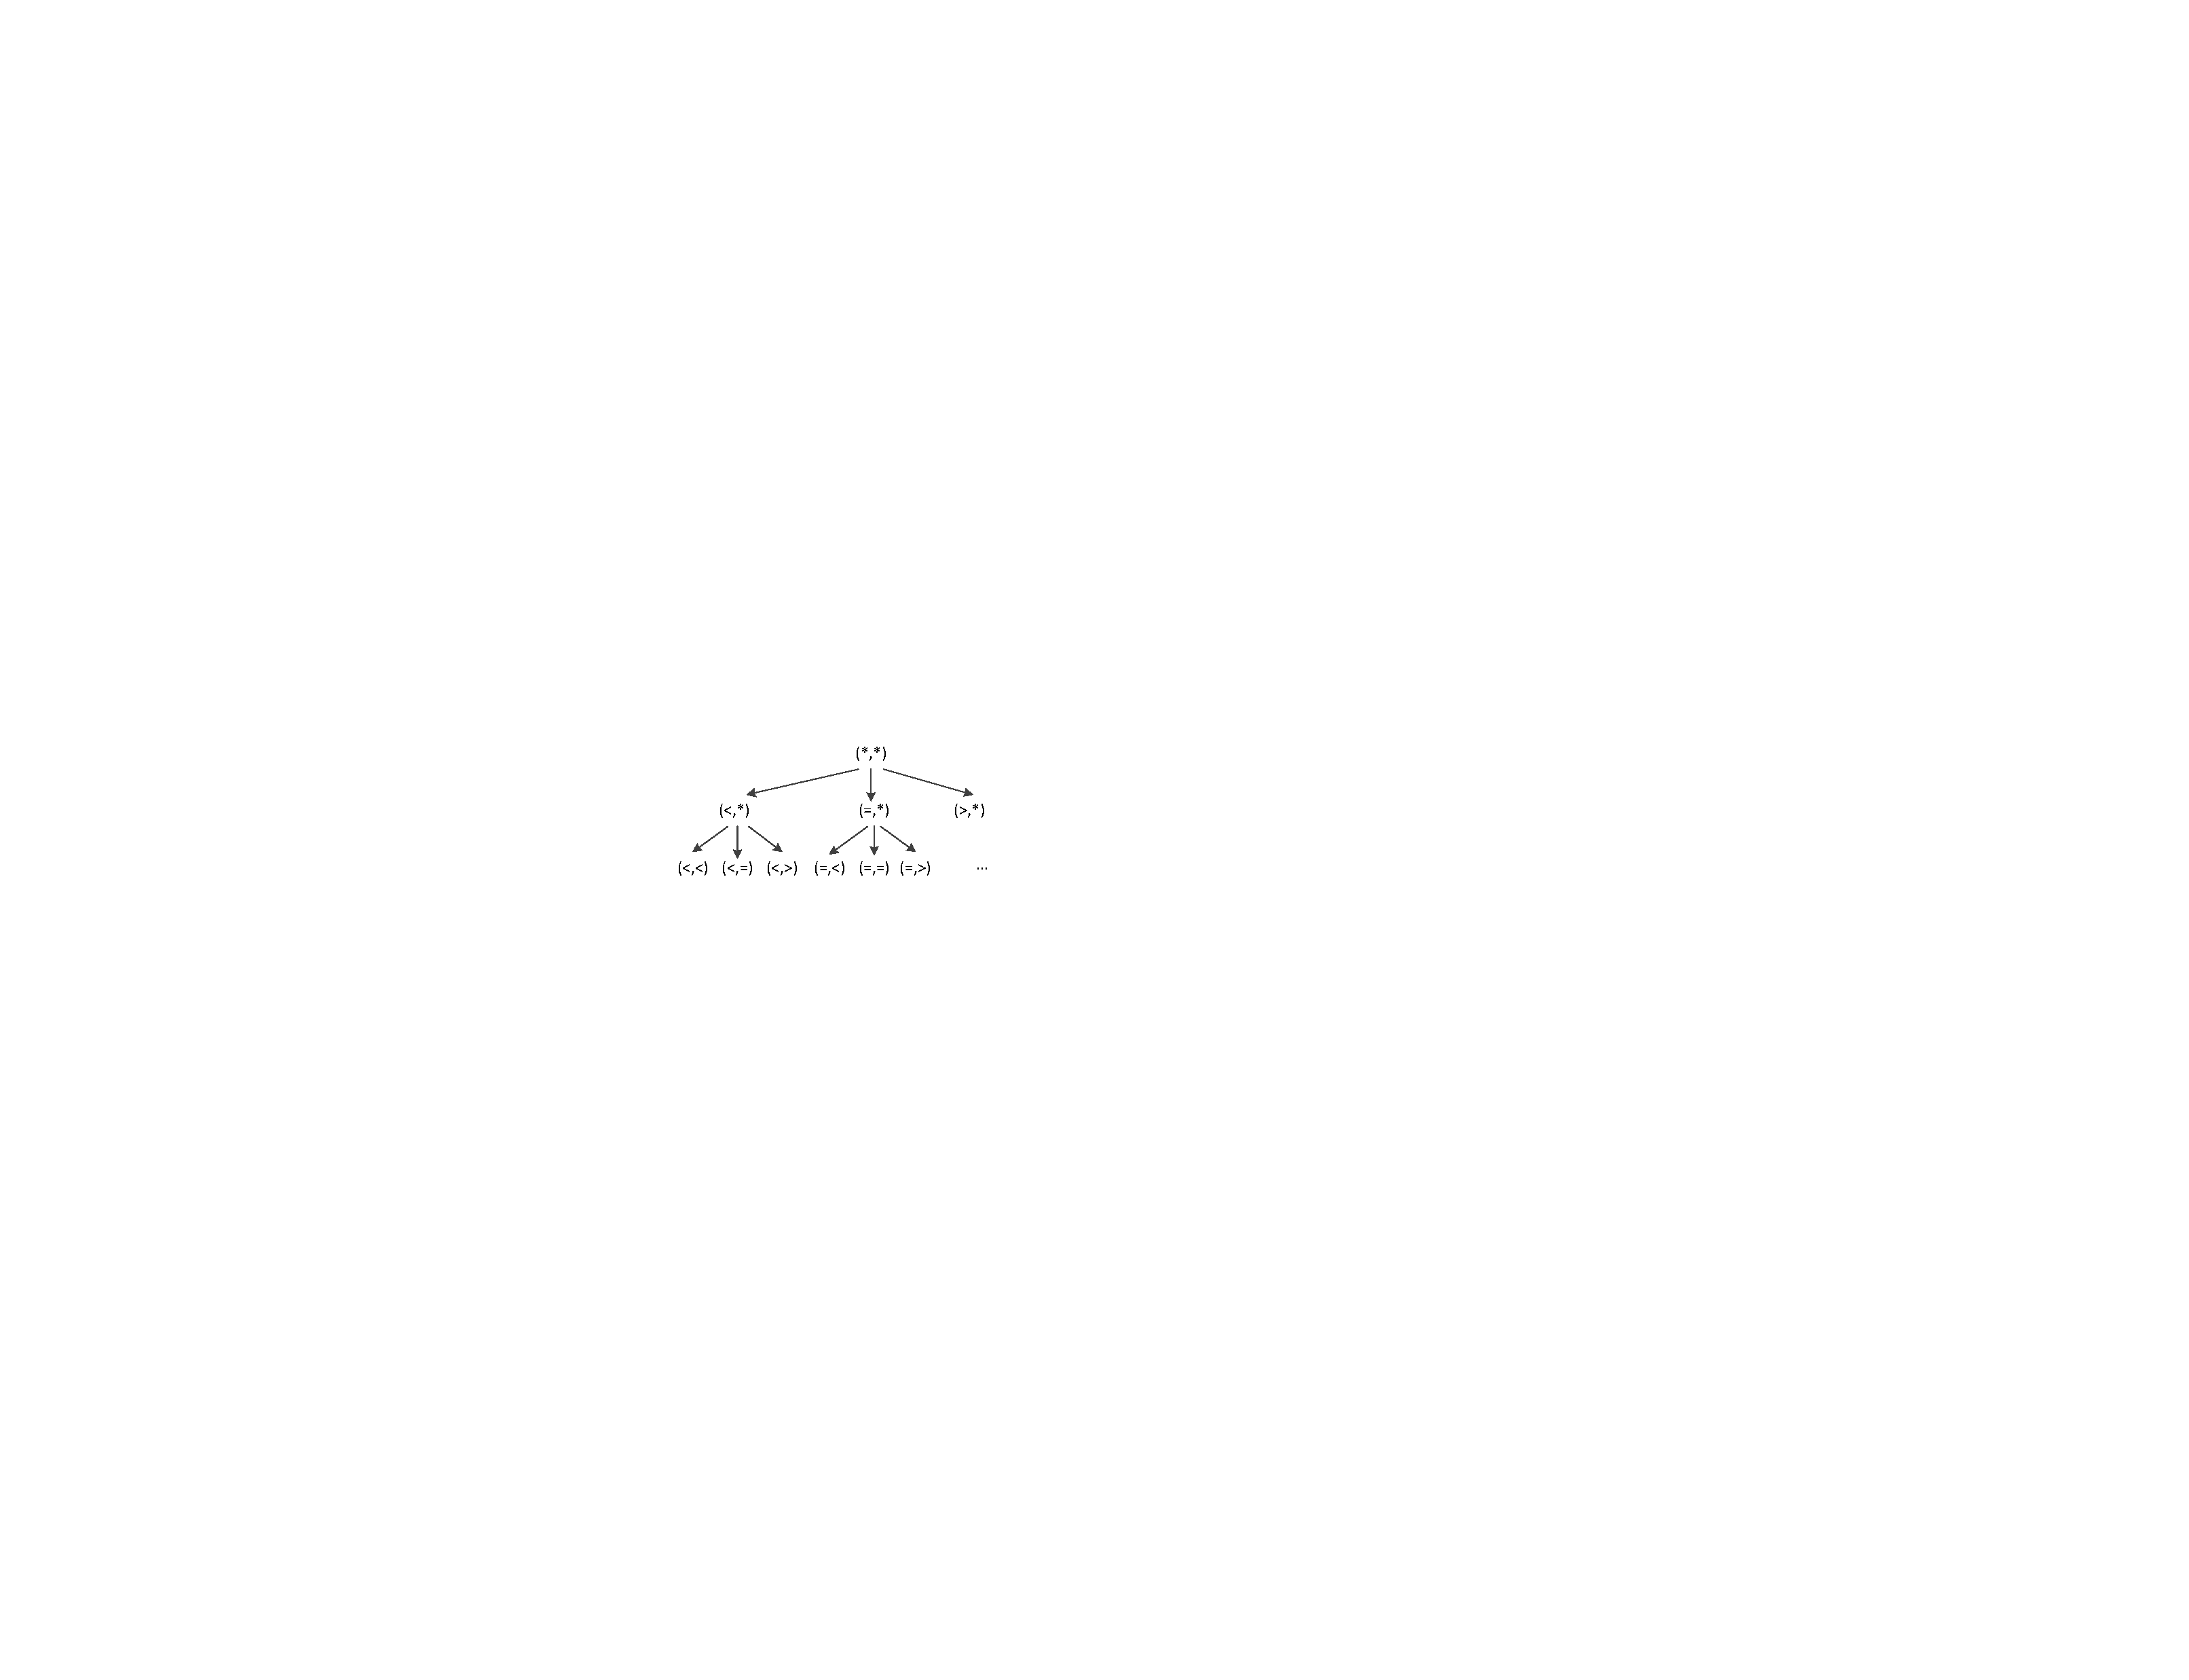
\includegraphics[width=0.6\linewidth]{chap6fig/testingHier.pdf}
\caption{Hierarchy of Dependency Testing for A Two-Level Loop Nest
\label{fig:testingHier}}
\end{center}
\end{figure}

During the \textit{offline phase}, when the direction vectors based off past runtime profiles are assumed to be true, various transformations are performed. If any of these
assumption is wrong, the generated accelerator will produce wrong results and should
not be run. The \textit{online phase} therefore needs to check these assumptions. More
specifically, it needs to check for the presence of any direction vectors which would
invalidate the reordering the \textit{offline phase} has performed. Table~\ref{} lists
all the tests we need to perform, given a particular transformation.


%These tests certainly introduce runtime overhead into our system. 
Depending on how much actual computation is going on in the target loop nest, these tests may be incurring a significant runtime overhead, especially if they are run on the processor. On the other hand, these tests are highly parallelizable and can be potentially
offloaded to the hardware completely. In either case, these checks reduce the overall
speed up attainable with the accelerator. Together with the cost of data transfer, which
will be described in section~\ref{dtransfer}, these overheads can nullify the benefit of computation offloading. Fortunately, we can statically devise a simple model to
evaluate if the amount of computation justifies the invocation of the validity check and
accelerator:

$R_t(I)  D_t + T_t$

$R_t(I)$ is a simple function estimating the reduction in execution time of the accelerated loop nest, given the size of the iteration space. Meanwhile $T_t$ and $D_t$ are functions
estimating the time used for data transfer and the parallelism validity check. This model is
generated during the offline phase and executed during the online phase. An example model
is shown in figure~\ref{}. Note how the model can be reduced to a set of quick checks
on the loop bounds, whose impact on execution time would be rather small.


The main steps for the execution of the accelerator-augmented program binaries is illustrated in figure~\ref{}. As the cost model is always evaluated, in the worst case, when
the accelerated version of the loop nest is never executed, there would be a slight reduction in performance. It is therefore advisable to only apply our approach to loop nests whose
past behavior exposes sufficiently sized iteration space.



%The performance estimates shown in figure~\ref{fig:fpgaparal} do not take into account the data access latency
%if they have to be brought in from off-chip RAM. By performing transformations
%to maximize data reuse, it can increase the ratio of computation v.s. off-chip memory bandwidth usage. 
\subsection{Data Transfer and Address Translation}
\label{dtransfer}
Another particular important aspect in ensuring the efficient execution of the accelerators is in the management of data transfers.
As the FPGA are used as an accelerator for binaries executed on CPU, the source
and final destination of its working datasets both are the address space of
the processor. Depending on the actual configuration of the system, the processor memory may or may not be directly accessible by the FPGA, as discussed in section~\ref{chartarg}. We thus need to provide mechanisms to enable
the sharing of data between the two substrates.


For the case where the FPGA can directly access the 
CPU memory, the easiest way is to apply the transformation and
optimizations described in chapter~\ref{decoupleChap}. This would
naturally create a set of address generators who pipeline requests into the 
memory subsystem, as can be seen from figure~\ref{}. To benefit from the locality-driven optimization we 
have performed, caches can also be inserted between the address outputs and the
off-chip memory. 


The regularity of the memory access patterns in our targeted loop nests
allows us to easily decouple the management of data transfer from the actual computation.
We can derive concise representations of the accessed addresses by the accelerator without actually running it. 
If the FPGA does not have direct access to the CPU memory, then explicit
data transfer is required. This is usually higher cost






Locality driven optimizations performed
described in section~\ref{}




The analyzability required for coarse grained parallelism discovery 
already provided us with 

also
facilitates the calculation of the exact memory footprint for the accelerated computation. 


More specifically, the addresses stream can be 




In addition, many processor centric systems 
use virtual memory to facilitate programming and manage the memory hierarchy, 






The approach described in chapter~\ref{decoupleChap} may be used but provides little advantage for these computation. 






 

%with 
%a particular parallel architecture as the target may be unnecessary. For %instance, vectorizing compilers may perform loop interchange to have 

%An interesting aspect of 

Our parallelization engine attempt to  

\begin{comment}
The variety of hardware templates gives another dimension in the accelerator design space, in addition to the software domain optimizations like loop interchange, loop tiling etc. 

For a specific loop nest, whose dependence graph is constructed using the information acquired through dependency analysis, there are multiple
possibilities 

As mentioned in section~\ref{sec:fdtp}, we use Banerjee's tests to find 
direction vectors between different statements in the loop nest. There are 
a few additional techniques employed to make runtime check cheaper
\end{comment}





One particular important aspect, in ensuring the efficient execution of the accelerators, is in the management of data transfers. 
The regularity of the memory access patterns in our targeted loop nests
allow us  to easily decouple the transfer of data from the computation. 
The analyzability required for coarse grained parallelism discovery also
facilitates the calculation of the exact memory footprint for the accelerated computation. More specifically, the addresses stream can be 


The approach described in chapter~\ref{decoupleChap} may be used but provides little advantage for these computation. 

\begin{comment}
At a high level, the approach we are proposing in accelerating program binaries
can be divided into two phases. For an acceleratable loop nest, we first examine
it's past execution profile to extract necessary information to perform dependency analysis offline. After obtaining the dependency direction vectors between statements, we can then perform parallelization and the actual accelerator synthesis. 
Now, whether the generated accelerator is consistent
with the semantics of the original program depends on if the dependency
testing results remain true when the actual execution happens. This is our
second phase, where an online check is performed to confirm the validity
of the assumed parallelism.
\end{comment}








\newpage


\newpage
\newpage
\section{Accelerator Integration through Binary Instrumentation}
\newpage

\section{Experimental Evaluation }
\label{biev}












\begin{comment}

%When the input data are changed, the generated accelerator may actually violate
%the semantics of the program. As we have mentioned in section~\ref{sec:cfbba},
%a verifying function is invoked before the accelerator to ensure the correctness
%of the overall execution. Besides, the \textit{online} phase also need to 



%Now the dependency testing results and the subsequent parallelization are a reflection of the programs' past behavior which
%may or may not hold true when the input data are changed. This is when the
%second phase 






%To actually obtain the direction vectors from equation~\ref{adioeq},
%we use Banerjee's approach~\cite{banerjee}.
%To actually solve equation~\ref{adioeq}, we use Banerjee's approach~\cite{}, which find the solution for the non-integer relaxation of the ILP formulation. It does
%which requires constant coefficients. 
%As the coefficients in the equation are not known from the static binary, our flow examines the runtime profiles to extract the values.
%The direction vectors thus obtained can be used evaluate how much coarse
%grained parallelism 



%Their values are extracted from the runtime profile of the programs.
Therefore, the dependency testing results are a reflection of the programs'
past behavior, which may or may not hold true when the input data are changed.
However, given a new set of runtime variables, the amount of computation needed to confirm the results of earlier dependency testing would be constant. This is not hard to see as the size of the problem formulated 
does not depend on the actual values of the coefficients. We now have the computation which has $O(1)$ cost yet guarantees the validity of the extracted
parallelism.


Meanwhile, it is worth noting that Banerjee's inequality only tests for existence of \textit{ real} solutions for the Diophantine's equations. Since it only tackles the non-integer relaxation of the ILP formulation, the results obtained are conservative. False dependencies are reported if all the real solutions are non-integral. More accurate tests like~\cite{omega} find integer solutions but are more costly. As we are
going to perform the test using runtime data when the accelerator is actually
being invoked, the faster, though more pessimistic, approach is preferred.





To actually obtain the direction vectors from equation~\ref{adioeq},
we use Banerjee's approach~\cite{banerjee}.
%To actually solve equation~\ref{adioeq}, we use Banerjee's approach~\cite{}, which find the solution for the non-integer relaxation of the ILP formulation. It does
%which requires constant coefficients. 
As mentioned in section~\ref{sec:cfbba}, the coefficients in the equation, despite being unchanged during the loop execution, are not known from the static binary. Our flow examines the runtime profiles to extract the coefficient values
%Their values are extracted from the runtime profile of the programs.
Therefore, the dependency testing results are a reflection of the programs'
past behavior, which may or may not hold true when the input data are changed.
However, given a new set of runtime variables, the amount of computation needed to confirm the results of earlier dependency testing would be constant. This is not hard to see as the size of the problem formulated 
does not depend on the actual values of the coefficients. We now have the computation which has $O(1)$ cost yet guarantees the validity of the extracted
parallelism.


Meanwhile, it is worth noting that Banerjee's inequality only tests for existence of \textit{ real} solutions for the Diophantine's equations. Since it only tackles the non-integer relaxation of the ILP formulation, the results obtained are conservative. It will never report lack of dependencies when one exists,  but may report false dependencies -- when all the real solutions are non-integral. More accurate tests like~\cite{omega} find integer solutions but are more costly. As we are
going to perform the test using runtime data when the accelerator is actually
being invoked, the faster, though more pessimistic, approach is preferred.







As we mentioned in section~\ref{sec:cfbba}, for loops with analyzable memory accesses, we can perform run time check to validate parallelization we performed in creating the accelerators. This 

As we use past execution profiles to extract parallelism and then perform runtime checks to confirm the validity of our parallelization, our approach
in accelerating program binaries can be divided into two phases. The offline
phase (compile time) consists of dependency analysis, accelerator synthesis and accelerator driver generation. Meanwhile, the parallelism validity check, data transfer and invocation of the accelerator are all performed during the online phase (run time). Being part of the driver, the actual code segments to perform validity check and data transfer are all generated during compile time. As our primary objective is to boost the performance of the accelerated loop nests, the flow tries to create simple and fast run time code whenever it, at the expense
of the compilation time and at times, the accuracy of the run time mechanisms.
\end{comment}